\documentclass{article}
\usepackage{amsmath}
\usepackage{amssymb}
\usepackage{enumerate}
\usepackage{graphicx}
\usepackage{caption}
\usepackage{float}
\usepackage{fullpage}
\usepackage{subcaption}

\begin{document}

\title{Follow the Sun: Learning North from Images}
\author{Brandon Minor \& Jack Morrison}
\maketitle

%%%%%%%%%%%%%%%%%%

\newcommand{\degrees}{$^\circ$ }

%%%%%%%%%%%%%%%%%%
\abstract{

Humans have navigated by the sun for millennia, relying on its predictable path across the sky to determine their own heading relative to north. We have applied Machine Learning algorithms to this practice in an attempt to do the same through images with only RGB data. Data was collected from three different areas in the US, all with different latitudes. A number of classification and regression algorithms were run on the different data sets, with varying success. 
%% Fill in more later
}

%%%%%%%%%%%%%%%%%%
\section{Experiment Setup}

%%
\subsection{Data Collection}
Datasets consisted of a series of images taken from one spot while rotating at least a full 360\degrees.
To train our parameters, our datasets need to include the heading and timestamp of every image. We produced an Android application to facilitate this process. Images were captured as fast as possible by the phone's camera and saved on external memory. Every photo taken had a related orientation vector that the phone registered at that timestamp. This vector was produced by the phone's magnetometer and registered the difference, in degrees, of the heading of the phone with respect to gravity and magnetic north. Images were only captured if the phone was nearly vertical, i.e.\ pitch of the phone was within $\pm$5\degrees of horizontal, as measured by the phone's internal sensors.

%%
\subsection{Programming}
All Machine Learning algorithms used (described in Section 3) were part of the scikit-learn toolkit for Python. scikit-learn also performed cross-validation on datasets provided. All plotting was done with the matplotlib library. 

%%%%%%%%%%%%%%%%%%
\section{Learning}

\begin{figure}[h!]
  \begin{subfigure}[!h]{0.5\textwidth}
    \centering
    \includegraphics[width=\textwidth]{./features_img.eps}
    \caption{Sample image from the Woodley Park dataset}
    \label{img:woodley_sample}
  \end{subfigure}
  \begin{subfigure}[!h]{0.5\textwidth}
    \centering
    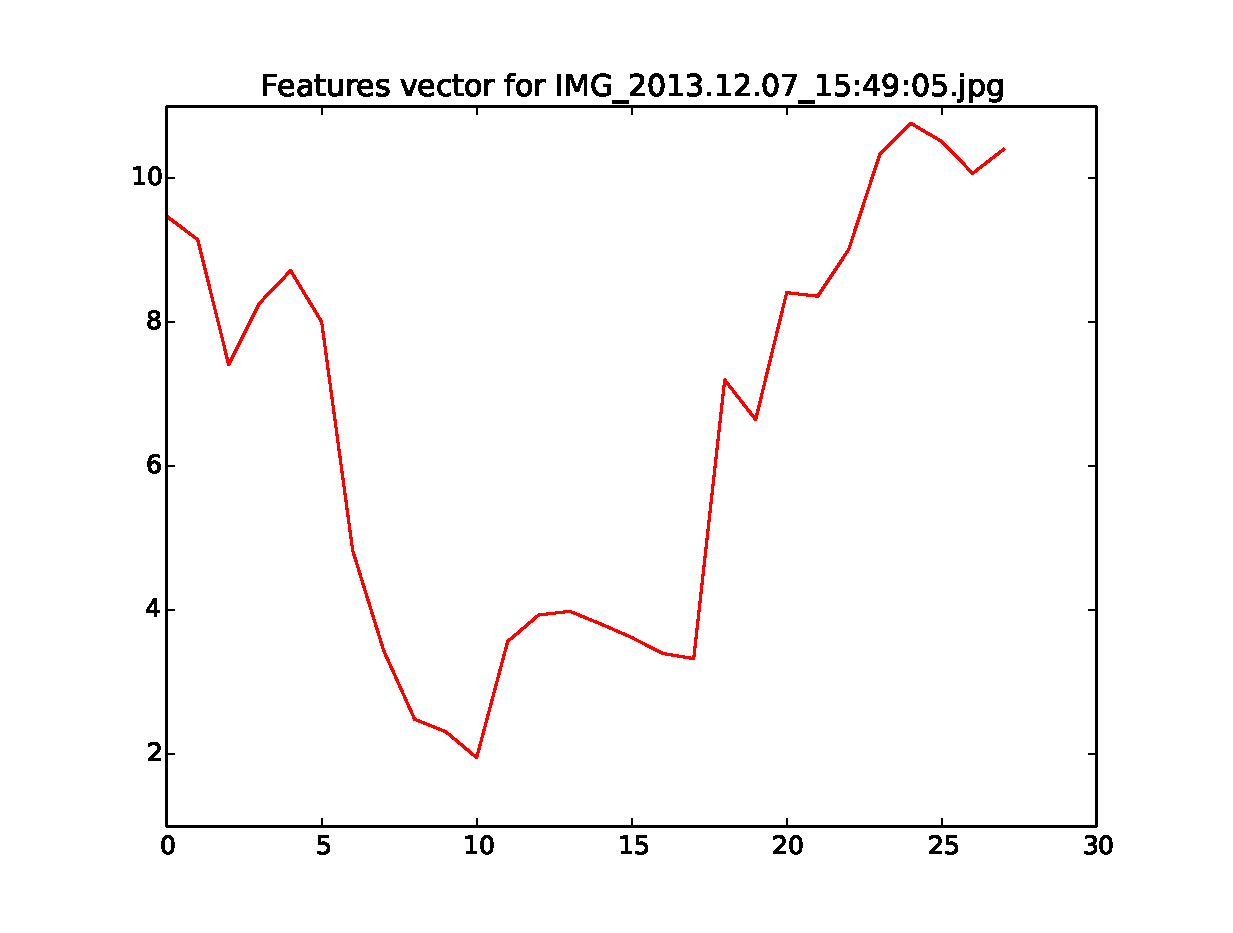
\includegraphics[width=\textwidth]{./Brightness_data.eps}
    \caption{Feature vector plot for image \ref{img:woodley_sample}}
    \label{img:woodley_features}
  \end{subfigure}
  \caption{Sample image and features used in learning}
\end{figure}

\subsection{Features}
Each image in our dataset has over 900,000 pixels so feature extraction is necessary. To use every pixel of every image as a feature for learning would not only be computationally infeasible, it would also make learning extremely difficult. We chose to use a simple image brightness-based feature set for this image. To compute the feature vector, each image was converted to grayscale and scaled to $18x10$. The columns and rows of this ``thumbnail'' image were then summed to produce a rough plot of the shape of the brightness through the image. These vectors (one for the column sums, one for the row sums) were then concatenated to produce the feature vector you can see in Figure \ref{img:woodley_features}.

\subsection{Cross-validation and Labeling}
Cross validation was performed on all datasets. After experimenting with both n-fold and leave-one-out validation, we used leave-one-out for all of our tests. 

Magnetometer data registered magnetic north as 0\degrees of yaw, with the degree increasing clockwise around the compass rose. The yaw of each image served as the training label used in every machine learning process.

%%
\subsection{Classifier Algorithms}
The main objective of this project is to formulate a reliable classifier; if we can label the orientation of one set of images with low range of error, we would hope the classifier would work similarly for other data sets. As such, each classifier breaks the 360 compass degrees into twelve 30-degree increments before analysis. We used two different algorithms for classification: 
\begin{enumerate}[1.]
\item Support Vector Machines - We used polynomiall radial basis function, and linear kernels. Since there were twelve different incriments, the SVM treated the dataset as having 12 distinct classes. 
\item Decision Forests
\end{enumerate}

%%
\subsection{Regression Algorithms}
Beyond this comparison of algorithms, we also performed regression function training. Our regression functions take our feature vectors and output an angle in degrees, with zero degrees being magnetic north. Our initial experiments used Linear Regression, using both LASSO and Ridge loss functions. 

%%%%%%%%%%%%%%%%%%
\section{Testing and Analysis}
\subsection{SVM - Linear kernel}
Linear kernel proved to be very unsuccessful for our purposes. Due to the non-linear nature of our data (See fig. 

\subsection{SVM - Ponynomial kernel, degree 3}

\subsection{SVM - RBF kernel}


\subsection{Linear Regression - LASSO vs. Ridge}



\subsection{Decision Trees}








%%%%%%%%%%%%%%%%%%
\section{Further Work}

%%
\subsection{More Features}

\begin{enumerate}[1.]
\item Histogram of Oriented Gradients (HOG): Bins of pixels are formed into histograms representing the gradient of brightness levels in the bin. Feature count is dependent on the size of the bin. 
\begin{figure}[H]
\centering
\setlength\fboxsep{2pt}
\setlength\fboxrule{0pt}
\fbox{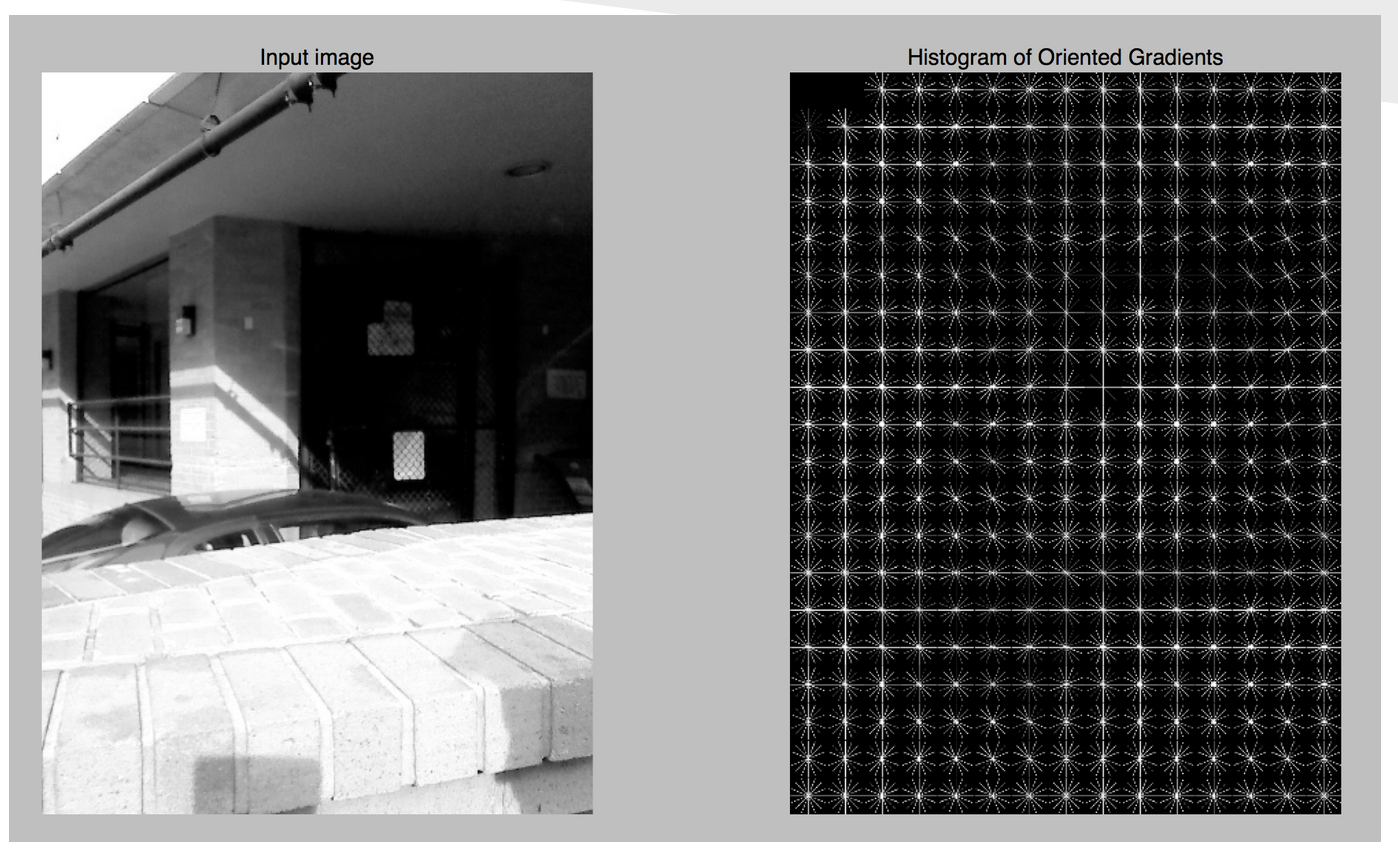
\includegraphics[scale=.3]{./HOGpic}}
\caption{
HOG
}
\end{figure}

\item RANSAC and shadow detection: using a point cloud of dark pixels, RANSAC is performed to get a basic linear function that fits the trend. This is then compared to other photos, and similar trends are classiied similarly.
\begin{figure}[H]
\centering
\setlength\fboxsep{2pt}
\setlength\fboxrule{0pt}
\fbox{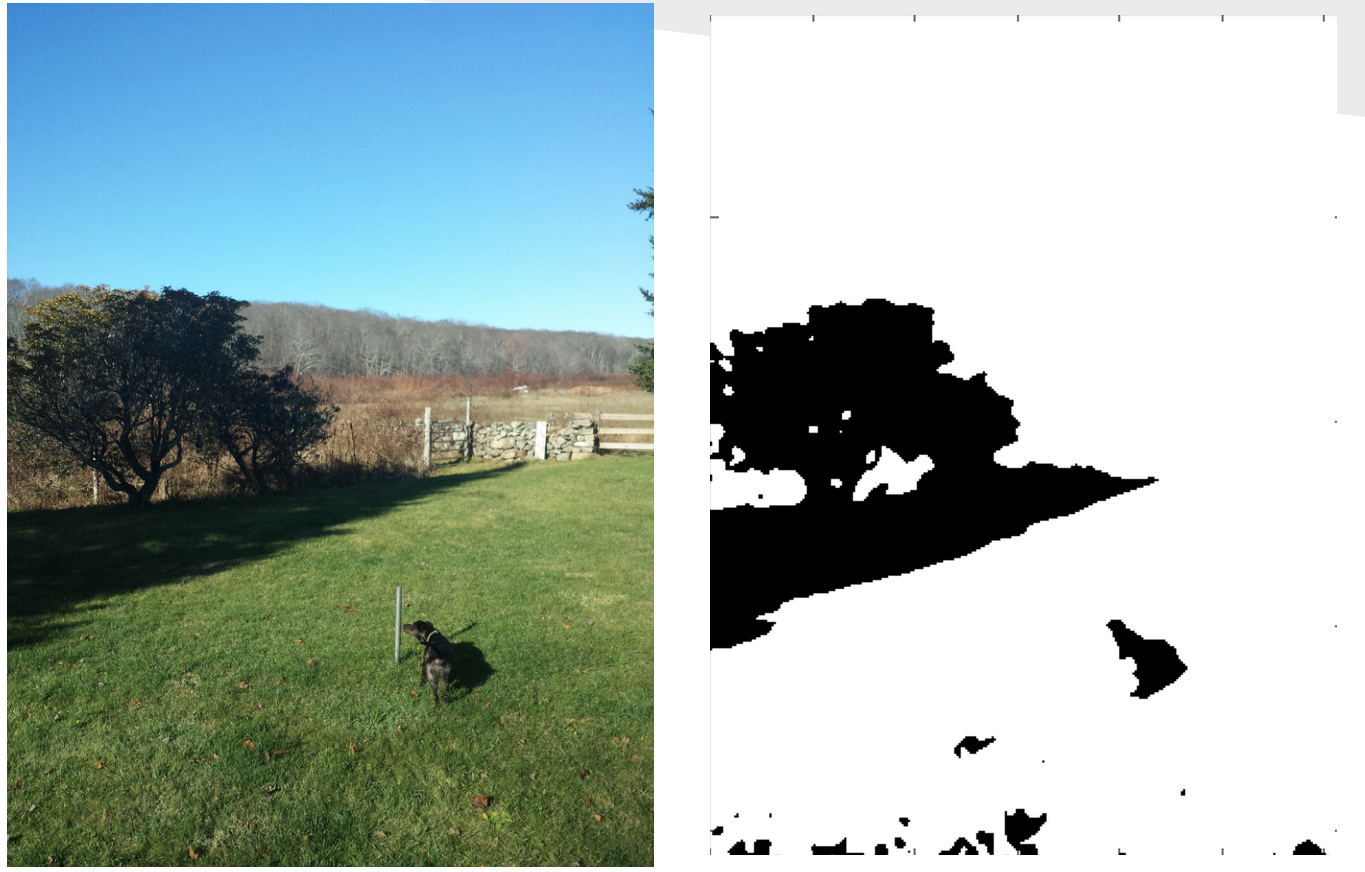
\includegraphics[scale=.3]{./RANSAC}}
\caption{
RANSAC (proposed)
}
\end{figure}

\end{enumerate}





\end{document}